\part{Equazioni Differenziali}
\chapter{Equazioni Differenziali}
\section{Preliminari}
Equazione è un uguaglianza in cui c'è almeno una incognita.\\
Equazione differenziale è un particolare tipo di equazione e stabilisce una relazione tra la funzione incognita e le sue derivate.In un equazione funzionale si cerca l'uguaglianza di: insieme di arrivo, insieme di partenza, corrispondenza.\\
Non è necessario sapere il valore della soluzione ma sapere che ne esiste una.????????\\\\
Equazione differenziale ordinaria:\\
1- La funzione incognita è funzione di una sola variabile, solitamente il tempo.\\
2- La funzione incognita e le sue derivate sono calcolate allo stesso istante di tempo.\\
\definition\label{def:equaz_diff}
Si dice equazione differenziale ordinaria di ordine $n$ nella funzione incognita $x\in \R^k$ un espressione del tipo:
$$f(t,x, x',\ldots,x^{(n)})=0$$
dove $f:A\to \R^m$, $A\subseteq \R^{1+(1+n)k}$ e $t\in \R$.\\
$m$ e $k$ caratterizzano il problema e son dunque libere. La dimensione di partenza $1+(1+n)k$ del problema è obbligata e dovuta alla somma di:
\begin{itemize}
	\item $1 = dim(t)$
	\item $(1+n)k$
	\begin{itemize}
		\item $(1+n)$ il numero totale delle funzioni: $n$ derivate ed $x$ stessa
		\item $k$ la dimensione dell'insieme di partenza di ogni funzione incognita
	\end{itemize}
\end{itemize}
Soluzione di questa equazione differenziale è una qualunque funzione $x:I\to \R^k$ definita su un intervallo $I\subseteq \R$, derivabile $n$ volte in $I$ e tale che $\forall t\in I$\\
$$(t,x, x',\ldots,x^{(n)}) \in A$$
$$f(t,x, x',\ldots,x^{(n)})=0$$
Soluzione massimale  di un equazione differenziale ordinaria è una soluzione $x_m:I_m\to \R^k$ tale che nessuna soluzione possa essere definita in un intervallo $I$ con $I_m\subseteq I$
\begin{note}
	Un'equazione differenziale ammette, in generale, infinite soluzioni.
\end{note}
\begin{note} \hypertarget{note:diff_eq_sol_definit_set}{}
	La soluzione di un'equazione differenziale può, analiticamente, essere definita su un intervallo $J\supset I$ ($I$ intervallo di definizione della funz. differenziale $f$). Non ha però senso considerare il suo comportamento al di fuori di $I$, in quanto non ha valore dal punto di vista del sistema. Per questo motivo $J$ sarà sempre considerato $J\subseteq I$
\end{note}
\begin{note}
	dalla definizione \ref{def:equaz_diff} segue che l'insieme di definizione della soluzione di un'equazione differenziale può essere solo un intervallo
\end{note}
\begin{example}
	Presa l'equazione differenziale $ x'=1$, essa è risolta da $x(t) = t + \alpha$ per ogni $\alpha\in\R$
\end{example}
\exercise
La soluzione di un'equazione differenziale ordinaria non può avere 3 asintoti.
\begin{solution}
	La soluzione $x$ è funzione continua. In quanto continua non può avere più di 2 asintoti verticali e in quanto funzione non può avere più di 2 asintoti orizzontali.
\end{solution}
\definition
un'equazione differenziale è in forma normale  se e solo se si presenta nella forma 
$$x^{(n)} = g(t,x, x',\ldots,x^{(n-1)})$$
\observation
lo studio di un'equazione differenziale ordinaria in forma non normale inizia generalmente con l'utilizzo del Teorema della Funzione Implicita insieme ai teoremi sulle equazioni differenziali ordinarie in forma normale
\proposition\label{prop:equaz_n_equival_1}
ogni equazione differenziale ordinaria in forma normale di ordine $n$ è equivalente a una equazione differenziale ordinaria in forma normale di ordine $1$, cioè in cui compaiono solamente derivate prime.
\begin{proof}
	Data l'equazione
	$$x^{(n)} = g(t,x, x', x'',\ldots,x^{(n-1)})$$
	sia $y$ il vettore $y = \rvect{x &  x' &  x'' & \ldots & x^{(n-1)}}$. Abbiamo ora che le componenti del vettore sono
	$$y_1=x\qquad y_2= x'\qquad y_3= x''\qquad \ldots\qquad y_n=x^{(n-1)}$$
	ed al contempo
	$$y_1'= x'=y_2\qquad y_2'= x''=y_3\qquad y_3'= x'''=y_4\qquad\ldots\qquad y_{n-1}'=x^{(n-1)}=y_n$$
	Cioè, differenziando l'$i-esimo$ elemento (funzione) del vettore $y$, mi "sposto" all'elemento (funzione) $i+1$ di $y$. A questo punto tutti gli elementi di $y$ sono equazioni differenziali del primo ordine.\\
	Quindi l'equazione può essere scritta come il seguente sistema del primo ordine
	$$\begin{cases}y_1'\quad=\quad y_2\\y_2'\quad=\quad y_3\\\vdots\\y_n'\quad=\quad g(t, y_1, y_2,\dots,y_n)\end{cases}$$
\end{proof}
\begin{example}
	CASO n=2\\
	abbiamo che $ x''=f(t,x, x')$\\
	introduco $ X'=\begin{bmatrix} x'\\ x''\end{bmatrix}$ e $X=\begin{bmatrix}x\\ x'\end{bmatrix}$\\
	quindi $ X'=f(t,X)$
\end{example}
\begin{definition}
	\label{def:prob_cauchy_ord_1}
	si dice problema di Cauchy del primo ordine il problema di determinare una soluzione di un'equazione differenziale ordinaria del primo ordine, soddisfacente ad una condizione iniziale.
	$$\begin{cases}x'=f(t,x)\\x(t_0)=x_0\end{cases}$$
	Dove $f:J\times A\to \R^n$, $J\subseteq \R$ è un intervallo, $t_0\in\circdot{J}$, $A\subseteq \R^n$, $x_0\in\circdot{A}$.\\
	Soluzione di un problema di Cauchy è una funzione $x:I\to \R^n$, definita in un intervallo $I$ contenente $t_0$ nella sua parte interna, quindi $t_0\in I\subseteq J$.\\
	Tale funzione $x$ è soluzione dell'equazione differenziale $x'=f(t,x)$ ed è tale che:
	\begin{enumerate}
		\item $x(t_0)=x_0$
		\item $x(I)\subseteq A$
		\item $x$ derivabile
	\end{enumerate}
	Quindi il problema di Cauchy aggiunge un vincolo ad un'equazione differenziale, così si isola una singola soluzione
\end{definition}
\begin{note}
	Si considera un intervallo perché l'idea è di studiare l'andamento nel tempo e sarebbe difficile far previsioni con "buchi" di tempo
\end{note}
\begin{note}
	La condizione $x(t_0) = x_0$ viene spesso definita condizione iniziale, malgrado la definizione \ref{def:prob_cauchy_ord_1} indichi che $t_0 \in \circdot{I}$, dunque a rigore non dovrebbe essere sulla frontiera di $I$. Questo è dovuto al fatto che, spesso, $t_0$ è proprio all'inizio dell'intervallo in cui si cerca la soluzione dell'equazione, ma i risultati esposti continuano a valere con piccole modifiche alle dimostrazioni.
\end{note}
\begin{definition}
	soluzione massimale di un problema di Cauchy è una soluzione $$x_M:I_M\mapsto R^k$$ tale che nessun'altra soluzione della stessa equazione possa essere definita in un intervallo $I$ con $I_M \subset I$. Quindi è la soluzione definita sull'intervallo maggiore possibile.
\end{definition}
\begin{definition}
	si dice problema di Cauchy di ordine $n$ il seguente problema:\\
	Determinare una soluzione di un'equazione differenziale ordinaria di ordine $n$ soddisfacente a $n$ condizioni iniziali:
	$$\begin{cases}
		x^{(n)}=f(t,x,x',\dotsc,x^{(n-1)})\\
		x(t_0)=\alpha_0\\
		x'(t_0)=\alpha_1\\
		\vdots\\
		x^{(n-1)}(t_0)=\alpha_{n-1}
	\end{cases}$$
\end{definition}
\begin{note}
	Le condizioni iniziali devono essere assegnate tutte nello steso istante.
\end{note}
\begin{example}
	il problema di Cauchy $$\begin{cases}x'=x\\x(0)=1\end{cases}$$
	ammette, tra le altre, anche le seguenti soluzioni, tecnicamente distinte tra loro
	$$\funcdef{f_1}t[\realintervalclose{-1}{1}]{\R}[e^t] \qquad \funcdef{f_2}t[\realintervalclose{-2}{10}]{\R}[e^t]$$
	La soluzione massimale è
	$$\funcdef{f_M}t[\R]{\R}[e^t]$$
	con intervallo di partenza $\R$, avente evidentemente diametro maggiore possibile.
\end{example}
\begin{proposition}
	ogni problema di Cauchy di ordine $n$ è equivalente ad un problema di Cauchy del primo ordine
	\begin{proof}
		Dalla \ref{prop:equaz_n_equival_1}
	\end{proof}
\end{proposition}
\begin{definition}[Equazione di Volterra]
	\label{def:equaz_volterra}
	Ogni problema di Cauchy del primo ordine con secondo membro continuo
	$$\begin{cases}x'=f(t,x)\\x(t_0)=x_0\end{cases}$$
	è equivalente ad un'equazione integrale del tipo
	$$x(t)=x_0+\int_{t_0}^{t}f(\tau,x(\tau))\integrald{\tau}$$
	Questa equazione viene denominata \textbf{equazione integrale di Volterra}.
	\begin{proof}
		Integrando ambo i membri della prima equazione del problema di ottiene:
		$$\int_{t_0}^{t}( x')\integrald{\tau}=\int_{t_0}^{t}(f(\tau,x(\tau)))\integrald{\tau}$$
		$$x(t)-x(t_0)=\int_{t_0}^{t}(f(\tau,x(\tau)))\integrald{\tau}$$
		$$x(t)=x_0+\int_{t_0}^{t}(f(\tau,x(\tau)))\integrald{\tau}$$
	\end{proof}
	\begin{note}
		\hypertarget{note:volterra_non_cont}
		Questa equazione ha senso anche per alcune funzioni $f$ non non continue, ma solo misurabili nel primo argomento. Ne consegue che nei Teoremi di esistenza ed unicità (locali/globali) l'ipotesi ``$f$ continua'' può essere sostituita da ``$f$ continua a tratti in $t, \forall x$, continua in $x$ e limitata''.
	\end{note}
\end{definition}

\begin{observation}
	in generale un problema si dice \textbf{ben posto} o \textbf{ben posto nel senso di Hadamard} ogniqualvolta la soluzione:
	\begin{enumerate}
		\item esiste
		\item è unica
		\item dipende con continuità dai dati
	\end{enumerate}
\end{observation}

\section{La Legge di Malthus}
Una popolazione, dotata di tutto il necessario per vivere e riprodursi, cresce secondo la legge di Malthus: la velocità di crescita della popolazione è proporzionale alla popolazione stessa.
$$ x'=k\cdot x$$
dove $x$ è il numero di membri della popolazione e $k$ è una costante positiva legata alla prolificità della specie in esame, generalmente calcolata come differenza tra i tassi di natalità e di mortalità.\\
Il problema di Cauchy è quindi
$$\begin{cases}
	x'=k\cdot x\\
	x(t_0)=x_0\\
\end{cases}
\qquad\text{con $x\in \R, k>0 $ e $ x_0=0$}$$

\begin{center}
	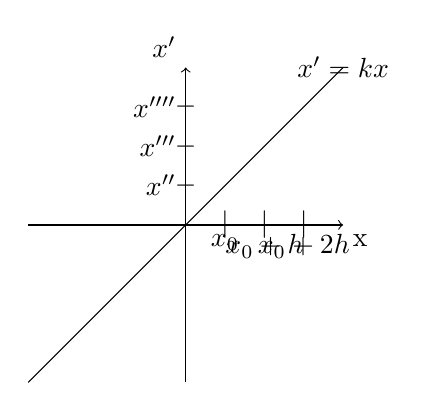
\begin{tikzpicture}[scale=1] %[x={10.0pt},y={10.0pt}]
	\pgfmathsetmacro\MAX{2}
	\draw[->] (-\MAX,0) -- (\MAX,0) node[anchor=north west] {x};
	\draw[->] (0,-\MAX) -- (0,\MAX) node[anchor=south east] {$ x'$};
	\draw[domain=-2:2,smooth,variable=\x] plot ({\x},{\x}) node {$ x'=kx$};
	\draw node at (0.5,0) {$|$};
	\draw node at (1,0) {$|$};
	\draw node at (1.5,0) {$|$};
	\draw node at (0,0.5) {$-$};
	\draw node at (0,1) {$-$};
	\draw node at (0,1.5) {$-$};
	\draw node[anchor=north] at (0.5,0) {$x_0$};
	\draw node[anchor=north] at (1,0) {$x_0+h$};
	\draw node[anchor=north] at (1.5,0) {$x_0+2h$};
	\draw node[anchor=east] at (0,0.5) {$ x'' $};
	\draw node[anchor=east] at (0,1) {$ x''' $};
	\draw node[anchor=east] at (0,1.5) {$ x''''$};
	
	\end{tikzpicture}% pic 1
	\qquad % <----------------- SPACE BETWEEN PICTURES
	\begin{tikzpicture}[scale=1] %[x={10.0pt},y={10.0pt}]
	\pgfmathsetmacro\MAX{2}
	\draw[->] (-\MAX,0) -- (\MAX,0) node[anchor=north west] {t};
	\draw[->] (0,-\MAX) -- (0,\MAX) node[anchor=south east] {x};
	\end{tikzpicture}% pic 2
\end{center}

blablabla ....\\
.......\\
Limiti di questo modello:
\begin{itemize}
	\item la variabile $x$ dovrebbe variare in $\N$, poiché una popolazione ha un numero intero di elementi.
	\item In molte specie è verosimile che il numero di nati al tempo $t$ dipenda dalla popolazione presente ad un tempo precedente $x(t-T), T>0$
	\item Supporre che una popolazione abbia per sempre a disposizione risorse sufficienti può non essere realistico
	\item Questo modello va bene quando si considerano intervalli di tempo molto lunghi.
\end{itemize}

\section{Teoria Locale}
\begin{definition}
	\label{def:loc_lips}
	Una funzione $f:I\times A\to \R^n$, con $I$ intervallo in $\R$ e $A$ aperto in $\R^n$, si dice \textbf{localmente lipshitziana} in $x\in A$ \textbf{uniformemente} rispetto a $t$ se
	$$\forall x_0 \in A, \exists r>0 e L>0: \forall x_1,x_2 \in (B(x_0,r)\cap A), \forall t\in I$$
	vale che
	$$\norm{f(t,x_2)-f(t,x_1)}\leq L\cdot\norm{x_2-x_1}\qquad o, ugualmente\qquad\frac{\norm{f(t,x_2)-f(t,x_1)}}{\norm{x_2-x_1}}\leq L$$
	Una funzione è uniformemente lipschitziana (\textbf{unif. lips.}) se, in parole povere, è possibile individuare un intervallo $I$ in cui il rapporto tra incremento del valore della $f$ e delle $x$ è minore di un valore fisso $L$ 
\end{definition}
\begin{note}
	La località è data da $x_1,x_2 \in (B(x_0,r)\cap A)$ e l'uniformità da $\forall t\in I$. Quindi la $f$ rimane lips. in modo uniforme al variare di $t$ (cioè $\forall t\in I$), ma questo non è garantito $\forall x\in A$, solo per $x_1,x_2 \in (B(x_0,r)\cap A)$.
\end{note}
\begin{note}
	\hypertarget{note:if_lips_then_loclips}
	Se $f$ \textbf{lips} su $A\implies f$ \textbf{loc. lips.} su A
\end{note}
\begin{proposition}
	\label{prop:fc1_loc_lips}
	Siano $I\subseteq \R$ un intervallo aperto e $A\subseteq \R^n$ un aperto. Ogni funzione $f\in\cntclass{1}(I\times A;\R^n)$ è loc. lips. in $x\in A$ uniformemente rispetto a $t\in I$
	\begin{proof}
		Il prodotto cartesiano $I\times A$, essendo prodotto cartesiano di aperti in $\R^n$ con metrica euclidea (si suppone sia in uso questa metrica), è a sua volta un aperto. Questo risultato è dovuto alla definizione stessa del prodotto cartesiano di $\R$ con metrica euclidea.\\
		% TODO scrivere proposizione poligonale capitolo 1. Magari anche proposizione prodotto cartesiano di aperti = aperto.
		Chiamiamo ora $S=I\times A$ l'insieme di partenza della $f$. Grazie alla \ref{prop:polig_cong_aperto} sappiamo che esiste una poligonale interamente contenuta in $S$ congiungente due qualunque punti dell'aperto $S$.\\
		È ora possibile applicare il \ref{teo:accresc_fin} ad uno qualunque dei segmenti formanti la poligonale appena individuata. Vale quindi la
		$$\norm{f(x_1)-f(x_0)}\le \sup\limits_{x\in S}\norm{Df(x)}\norm{x_1-x_0}$$
		che è direttamente comparabile alla definizione di locale lipschitzianità \ref{def:loc_lips} della funzione in ciascuno dei segmenti della poligonale, da cui la tesi.
	\end{proof}
\end{proposition}
\begin{example}
	La funzione $f:\R\mapsto\R$ data da $f(x)=x^2$ è \textbf{loc. lips.} su $\R$ ma non è \textbf{globalmente lips.} su $\R$. Vedasi \ref{def:fun_lips}
\end{example}

\subsection{Esistenza e Unicità}
\begin{proposition}[Teorema di Peano]
	\label{teo:peano}
	Si consideri il seguente problema di Cauchy:
	$$\left\{\begin{matrix} x'=f(t,x)\\x(t_0)=x_0\end{matrix}\right.$$
	con $f:I\times A\in \R^n$ soddisfacente alle ipotesi:
	\begin{enumerate}
		\item $t_0\in \circdot{I}, x_0\in \circdot{A}$
		\item $f\in \cntclass{0}(I\times A;R^n)$
	\end{enumerate}
	inoltre $I\subseteq \R$ intervallo e $A\subseteq \R^n$, in quanto \hyperref[def:prob_cauchy_ord_1]{problema di Cauchy}.\\
	Allora esiste un $\delta>0$ tale che esiste soluzione $x:J\mapsto A$ del problema di Cauchy con $J=\realintervalclose{t_0-\delta}{t_0+\delta}$.
	\begin{note}
		$\delta$ è un valore arbitrario che serve ad identificare l'intervallo $I$ a cui appartiene $t_0$
	\end{note}
	\noindent Inoltre:
	\begin{itemize}
		\item $J\subseteq I$ da \hyperlink{note:diff_eq_sol_definit_set}{nota definizione 47}, dunque $\varphi(J)\subseteq A$
		\item $\varphi(t_0)=x_0$
		\item $\varphi$ derivabile e $\varphi'(t)=f(t,\varphi(t))$
	\end{itemize}
	\begin{proof}
		Non richiesta
	\end{proof}
\end{proposition}
\begin{example}[Il Baffo/Pennello di Peano] % TODO da rivedere
	$$\left\{\begin{matrix} x'=\sqrt{\abs{x}}\\x(0)=x_0\end{matrix}\right.$$
	\begin{center}
		\begin{tikzpicture}[scale=1] %[x={10.0pt},y={10.0pt}]
		\pgfmathsetmacro\MAX{2}
		\draw[->] (-\MAX,0) -- (\MAX,0) node[anchor=north west] {x};
		\draw[->] (0,-\MAX) -- (0,\MAX) node[anchor=south east] {$ x'$};
		\draw[domain=0:2,smooth,variable=\x] plot ({\x},{(\x)^(1/2)});
		\draw[domain=-2:0,smooth,variable=\x] plot ({\x},{(-\x)^(1/2)});
		%\draw node at (0.5,0) {$|$};
		%\draw node at (1,0) {$|$};
		%\draw node at (1.5,0) {$|$};
		%\draw node at (0,0.5) {$-$};
		%\draw node at (0,1) {$-$};
		%\draw node at (0,1.5) {$-$};
		%\draw node[anchor=north] at (0.5,0) {$x_0$};
		%\draw node[anchor=north] at (1,0) {$x_0+h$};
		%\draw node[anchor=north] at (1.5,0) {$x_0+2h$};
		%\draw node[anchor=east] at (0,0.5) {$ x'' $};
		%\draw node[anchor=east] at (0,1) {$ x''' $};
		%\draw node[anchor=east] at (0,1.5) {$ x''''$};
		
		\end{tikzpicture}% pic 1
		\qquad % <----------------- SPACE BETWEEN PICTURES
		\begin{tikzpicture}[scale=1] %[x={10.0pt},y={10.0pt}]
		\pgfmathsetmacro\MAX{2}
		\draw[->] (-\MAX,0) -- (\MAX,0) node[anchor=north west] {t};
		\draw[->] (0,-\MAX) -- (0,\MAX) node[anchor=south east] {x};
		\end{tikzpicture}% pic 2
	\end{center}
	Se $x_0 = 0$ ho che $\varphi(t)=0$ è soluzione $\forall t$\\
	Ma $x' = \sqrt{\abs{x}}$ è anche un'equazione a variabili separabili, quindi risolvibile.
	$$\frac{x}{\sqrt{\abs{x}}}=1 \Rightarrow \int_{0}^{t}{\frac{ x'}{\sqrt{\abs{x}}}\integrald{t}} = t$$
	$$\int_{x(0)=0}^{x(t)}{\frac{1}{\sqrt{\abs{x}}}\integrald{x}} = t$$
	valuto ora il caso $x\geq0$, quindi $\abs{x}=x$
	$$\int_{x(0)=0}^{x(t)}{\frac{1}{\sqrt{x}}\integrald{x}} = 2\sqrt{x} = t$$
	La soluzione cercata è quindi $x(t)=\frac{1}{4}t^2$, estendendo il ragionamento ai tempi negativi si trova che la soluzione cercata è: $$\varphi(x)= \left\{\begin{matrix}+\frac{1}{4}t^2&&t>0,\\0&&t=0\\-\frac{1}{4}t^2&&t<0\end{matrix}\right.$$
	Abbiamo trovato che per la condizione iniziale $x_0=0$ il sistema ammette due soluzioni, si riesce estendere la soluzione a infinite funzioni.
	$$\varphi(x)= \left\{\begin{matrix}-\frac{1}{4}(t-a)^2&&t<a,\\0&&t\in[a,b]\\+\frac{1}{4}(t-b)^2&&t>b\end{matrix}\right.$$
	infatti:
	$$\varphi'(t) = \left\{\begin{matrix}-\frac{1}{8}(t-a)&&t<a,\\0&&t\in[a,b]\\+\frac{1}{8}(t-b)&&t>b\end{matrix}\right.$$ $$\left\{\begin{matrix}-\frac{1}{8}(t-a)=\frac{-\frac{1}{4}(t-a)^2}{	\sqrt{-\frac{1}{4}(t-a)^2}}&&t<a,\\0=0&&t\in[a,b]\\+\frac{1}{8}(t-b)=\frac{\frac{1}{4}(t-b)^2}{\sqrt{\frac{1}{4}(t-b)^2}}&&t>b\end{matrix}\right. = ....????? sistema $$
	Abbiamo quindi trovato infinite soluzioni.\\
	Questo esempio per sottolineare che il teorema di Peano non garantisce l'unicità della soluzione
\end{example}
\begin{example}[Continuità ed ipotesi necessaria] % TODO da rivedere
	Questo esempio mostra che se non c'è continuità, può?????????? non esserci la soluzione.\\
	Dato il seguente problema di Cauchy: $\left\{\begin{matrix}
	x' = \left\{\begin{matrix}1&&x<0\\-1&&x\ge 0\end{matrix}\right.\\
	x(0)=0
	\end{matrix}\right.$\\
	\begin{center}
		\begin{tikzpicture}[scale=1] %[x={10.0pt},y={10.0pt}]
		\pgfmathsetmacro\MAX{2}
		\draw[->] (-\MAX,0) -- (\MAX,0) node[anchor=north west] {x};
		\draw[->] (0,-\MAX) -- (0,\MAX) node[anchor=south east] {$ x'$};
		\draw[domain=0:2,smooth,variable=\x] plot ({\x},{1});
		\draw[domain=-2:0,smooth,variable=\x] plot ({\x},{-1});
		\draw node at (0,-1) {$\bullet$};
		\draw node at (0,1) {$\circ$};
		\end{tikzpicture}% pic 1
	\end{center}

	\noindent $x(t)=0$ soddisfa la condizione iniziale ma ovviamente non può essere soluzione del problema poiché per $x\ne 0$ si ha che $ x'=\pm 1$ che non è la derivata della funzione nulla.\\
	partendo sempre dalla condizione iniziale si può ipotizzare per esempio che la soluzione cresca, solo che questo contraddice $ x'(0)=-1$\\
	se invece si ipotizza che decresce da $0$ si ottiene che la funzione assume valori negativi, anche questo è un assurdo poiché la derivata per valori negativi della funzione è positiva.\\
	Precisiamo che se il problema fosse stato $\left\{\begin{matrix}
	x' = \left\{\begin{matrix}1&&x<0\\-1&&x\ge 0\end{matrix}\right.\\
	x(0)=-3\end{matrix}\right.$ allora la funzione $\varphi(x)=-x+3$ sarebbe stata soluzione nell'intervallo $J=\left] -\infty,0 \right[ $
\end{example}

\begin{theorem}[Teorema di Cauchy Locale]
	\label{teo:cau_locale}
	In sostanza si dimostra che il problema di Cauchy è ben posto nel senso di Hadamard.\\
	Si consideri il problema di Cauchy:
	$$\begin{cases}x'=f(t,x)\\x(t_0)=x_0\end{cases}$$
	con $f:I\times A \to \R^n$ soddisfacente le ipotesi:
	\begin{enumerate}
		\item $t_0\in \circdot{I}, x_0\in \circdot{A}$. Inoltre da \ref{def:equaz_diff} e note successive: $I$ intervallo e $I\subseteq \R^n$, inoltre $A\subseteq \R^n$
		\item $f\in \cntclass{0}(I\times A; \R^n)$ 
		\item $f$ è localmente Lipschitziana in $x\in A$ uniformemente rispetto a $t\in I$
	\end{enumerate}
	\begin{note}
		Le prime due ipotesi garantiscono l'esistenza, grazie al Thm. di Peano. La terza ipotesi rende il teorema più restrittivo, ma permette anche di giungere ad una conclusione più forte (ed utile).
	\end{note}
	\begin{note}
		Per verificare l'ultima ipotesi si ricordino \ref{prop:fc1_loc_lips} e \hyperlink{note:if_lips_then_loclips}{se $f$ \textbf{lips.} $\implies f$ \textbf{loc. lips.}}
	\end{note}
	Allora ho i seguenti risultati:
	\begin{enumerate}
		\item \textbf{Esistenza} (da \ref{teo:peano}): $\exists \delta>0$ con cui si identifica un $J=\realintervalclose{t_0-\delta}{t_0+\delta}$, inoltre $\exists\,\varphi : J \to \R^n$ soluzione con le proprietà date da Peano:
		\begin{itemize}
			\item $J\subseteq I$ da \hyperlink{note:diff_eq_sol_definit_set}{nota definizione 47}, dunque $\varphi(J)\subseteq A$
			\item $\varphi(t_0)=x_0$
			\item $\varphi$ derivabile e $\varphi'(t)=f(t,\varphi(t))$
		\end{itemize}
		\item \textbf{Unicità}\\
		Se $\exists\,J_1,J_2$ intervalli con $J_1\subseteq I,J_2\subseteq I$ e $\exists\,\varphi_1:J_1\to \R^n, \varphi_2:J_2\to \R^n$ soluzioni con le seguenti proprietà
		\begin{itemize}
			\item $J_1\subseteq I$, $J_2\subseteq I$ da \hyperlink{note:diff_eq_sol_definit_set}{nota definizione 47}, dunque $\varphi_1(J_1)\subseteq A$ e $\varphi_2(J_2)\subseteq A$
			\item $\varphi_1(t_0)=x_0,\,\varphi_2(t_0)=x_0$
			\item $\varphi_1,\varphi_2$ derivabili e
				$\begin{cases}
					\varphi_1'(t)=f(t,\varphi_1(t))\,\forall t \in J_1\\
					\varphi_2'(t)=f(t,\varphi_2(t))\,\forall t \in J_2
				\end{cases}$
				NB. Non è effettivamente sistema
		\end{itemize}
		\begin{note}
			Si può osservare che, sicuramente, $J_1\cap J_2\neq\emptyset$, poiché entrambi gli insiemi contengono almeno $t_0$ nella loro parte interna.
		\end{note}
		Allora $\varphi_1(t)=\varphi_2(t)$ $\forall t \in(J_1\cap J_2)$\\
		Cioè, se esistono due soluzioni, allora esse coincidono ovunque siano entrambe definite.
		\item \textbf{Dipendenza continua dai dati}\\
		Si considerino i seguenti problemi di Cauchy con condizione iniziale individuata nello stesso istante:
		$$(1)\begin{cases}x'=f(t,x)\\x(t_0)=x_0\end{cases}\qquad
		(2)\begin{cases}y'=g(t,y)\\y(t_0)=y_0\end{cases}$$
		con $f,g:I\times A \to \R^n$ e soddisfacenti le ipotesi di questo teorema.\\
		Allora esiste un $\delta >0$ tale che sull'intervallo $\realintervalclose{t_0-\delta}{t_0+\delta}$ sono definite una soluzione $\varphi$ di (1) ed una soluzione $\psi$ di (2). Inoltre esiste $L>0$ t.c. $\forall t\in \realintervalclose{t_0-\delta}{t_0+\delta}$ vale:
		$$\norm{\varphi(t)-\psi(t)} \le (\norm{x_0-y_0}+\delta\norm{f-g}_{\cntclass{0}})e^{L\abs{t-t_0}}$$
		dove $\norm{f-g}_{\cntclass{0}}=\sup\limits_{I\times A}\norm{f(t,x)-g(t,x)}$
		\begin{note}
			Questo significa che, con problemi diversi tra loro, se ($x_0$ e $y_0$), ($f$ e $g$) sono vicine tra loro ("a coppie"), allora sono vicine anche le soluzioni, ma per $t$ vicine.
			Pensando $t$ come tempo, cioè una delle applicazioni più classiche, questo implica che non si possano fare previsioni a lungo termine con sistemi diversi.
		\end{note}
	\end{enumerate}
\end{theorem}
\begin{note}
	Norma dell'integrale $\leq$ integrale della norma.
	$$\norm{\int{\cdot}\integrald{\cdot}}\leq\int{\norm{\cdot}\integrald{\cdot}}$$
\end{note}

\proposition LEMMA DI GRONWALL\\
Dati $a,b\in \R$ con $a\le b$ siano $\delta_0\in \left[ 0;+\infty \right]$ e $\delta,\kappa:\left[a,b\right]\to \R$ funzioni continue su $\left[a,b\right]$ con $\delta(t)\ge 0$,$\kappa(t)\ge 0 \quad \forall t\in\left[ a,b\right] $ e $\delta(t)\le \delta_0+\int_{a}^{t}\kappa(\tau)\delta(\tau)\integrald{\tau}$Allora $$\delta(t)\le\delta_0e^{\int_{a}^{t}\kappa(\tau)\integrald{\tau}}$$
Questo teorema porta da una stima implicita di $\delta$(sotto il segno di integrale) ad una stima esplicita 
\begin{proof}
	sia $\delta_0 > 0$. Sia $\Delta(t)=\delta_0+\int_{a}^{t}\kappa(\tau)\delta(\tau)\integrald{\tau}$.\\
	Vale per ipotesi che $\delta(t)\le\Delta(t)=\delta_0+\int_{a}^{t}\kappa(\tau)\delta(\tau)\integrald{\tau}$\\
	Sfruttando la derivata di $ln(\Delta(t))$ si ottiene $\frac{d}{\integrald{t}}(ln(\Delta(t)))= \frac{\Delta'(t)}{\Delta(t)}=\frac{\kappa(t)\delta(t)}{\Delta(t)}$, ed il termine $\frac{\delta(t)}{\Delta(t)}\le 1$, Integrando il primo e l'ultimo termine
	$$\int_{a}^{t}\left( \frac{d}{\integrald{t}}\left(ln(\Delta(t))\right) \right)\le\int_{a}^{t}\kappa(\tau)\integrald{\tau}$$
	$$ln(\Delta(t))\le ln(\delta_0)+\int_{a}^{t}\kappa(\tau)\integrald{\tau}$$
	$$ \Delta(t)\le\delta_0e^{\int_{a}^{t}\kappa(\tau)\integrald{\tau}} $$
	Da cui la tesi.
	Se $\delta_0=0$, ponendo $\Delta(t)=\epsilon+\int_{a}^{t}\kappa(\tau)\delta(\tau)\integrald{\tau}$ si ottiene $\delta(t)\epsilon$
\end{proof}

\begin{proof}(\textbf{Tesi 2})
	\begin{note}
		L'idea alla base della dimostrazione è che vogliamo riuscire a trasformare il problema di Cauchy in un problema di punto fisso mediante una funzione avente come parametro $x$ stesso.
	\end{note}
	Da \ref{def:equaz_volterra} sappiamo che la prima equazione del problema in ipotesi corrisponde all'integrale
	$$x(t)=x_0+\int_{t_0}^{t}(f(\tau,x(\tau)))\integrald{\tau}$$
	Definiamo quindi $T$, funzione del tipo
	\begin{equation}
		\label{equaz:cauch_proof_T}
		\funcdef{\textrm{$T$}}{(T(x))(t)}{X}[x_0+\int_{t_0}^tf(\tau,x(\tau))\integrald{\tau}]		
	\end{equation}
	Abbiamo così ottenuto un problema di punto fisso ($x=T(x)$). Ora bisogna determinare l'insieme di partenza e l'insieme di arrivo in maniera utile per la dimostrazione. Per poter applicare il \hyperref[teo:contrazioni]{Teorema delle contrazioni} serve che lo spazio di partenza e di arrivo corrispondano.\\
	Prendiamo:
	\begin{itemize}
		\item $\delta_1>0$ tale che $\realintervalclose{t_0-\delta_1}{t_0+\delta_1}\subseteq I$
		\item $\rho>0$ tale che $\overline{B(x_0,\rho)}\subseteq A$
		\item $L$ costante di Lipshitz di $f$ in $\realintervalclose{t_0-\delta_1}{t_0+\delta_1}\times\overline{B(x_0,\rho)}$. È possibile individuare $L$ in quanto $f$ loc. lips. per ipotesi in $I\times A$, e dunque \textbf{loc. lips. in sottointervalli/insiemi}
	\end{itemize}
	Sia ora
	$$V = \sup\brackets{\norm{f(t,x)}\,:\,t\in\realintervalclose{t_0-\delta_1}{t_0+\delta_1},x\in\overline{B(x_0,\rho)}}$$
	\begin{note}
		V è il massimo valore assunto dalla derivata prima ($x'=f(t,x))$) di una qualsiasi delle soluzioni $x$ contenute nella sfera $\overline{B(x_0,\rho)}$. È massimo di funzione continua (per ipotesi 2) in un compatto (per ipotesi 1, essendo in $\R^n\times\R^n$ e per \ref{prop:int_compatto}).\\% TODO in cap. 1, prop 2.35: compatto <=> chiuso+limtato (intervallo)
	\end{note}
	\noindent Definiamo dunque un generico $\delta>0$
	$$\delta<\min\brackets{\delta_1,\frac{\rho}{V},\frac{1}{L}}$$
	\begin{note}
		$\delta$ è strettamente minore del $\min$ perché poi servirà a trovare una contrazione, dunque dovrò avere sicuramente $\delta L < 1$
	\end{note}
	\begin{itemize}
		\item $\delta_1$ è raggio di un generico intervallo incluso in $I$ di partenza. $\delta$ deve essere minore di $\delta_1$ in quanto non è possibile uscire dall'intervallo $I$
		\item $\frac{\rho}{V}$ è rapporto tra il raggio di $\overline{B(x_0,\rho)}$, sfera interamente contenuta in $A$, e $V$, valore massimo di $f$ ridotta all'intervallo di cui sopra e alla sfera $\overline{B}$.\\
		Considerando il reciproco $\frac{V}{\rho}$, possiamo vederlo come una sorta di nuova costante di lips., riportata ad un intervallo più piccolo, non dipendente però da $\Delta f(x)$, ma dal valore di $f(x)$ stessa.
		\item $1/L = \frac{\norm{x_2-x_1}}{\norm{f(t,x_2)-f(t,x_1)}}$ dalla \ref{def:loc_lips}, perché $f$ loc. lips. per ipotesi. Dà un'idea di quanto vari la $x$ rispetto alla variazione della $f(x)$
	\end{itemize}
	Questo $\delta$, dunque, rappresenta, dal punto di vista concettuale, quale sia la più restrittiva ($\min$) tra tutte le possibili variazioni della $f(x)$ rispetto alla $x$.\\
	A questo punto, usando $\delta$, definiamo lo spazio $X$, generato da tutte le funzioni continue sul nuovo intervallo a valori entro una sfera centrata in $x_0$ con lo stesso raggio di $\overline{B}$
	$$X = \brackets{g\in \cntclass{0}(\realintervalclose{t_0-\delta}{t_0+\delta};\R^n):\forall t\norm{g(t)-x_0}\leq \rho}$$
	\begin{note}
		Si scelgono le funzioni continue ($\in \cntclass{0}$) perché serve $x$ continua per rendere valida l'equivalenza della funzione di Volterra con il problema di Cauchy. Stando alla \hyperlink{note:volterra_non_cont}{nota alla definizione di equazione di Volterra} sarebbe possibile sceglierla non continua, ma non si considera il caso.
	\end{note}
	Possiamo passare al punto chiave della dimostrazione, verifichiamo le ipotesi del \hyperref[teo:contrazioni]{Teorema delle contrazioni}:
	\begin{itemize}
		\item $(X,d)$ è \textbf{spazio metrico completo}\\
		$(X,d_X)$ è spazio metrico completo se considerato con la distanza della convergenza uniforme $d_X$ per la \ref{prop:compl_dist_conv}.\qed
		\item $T$ è \textbf{definita} (è possibile calcolarla)\\
		L'abbiamo definita all'inizio dall'equazione di Volterra\qed
		\item $T$ è \boldmath$X\mapsto X$\unboldmath\\
		L'insieme di partenza è valido in quanto sottoinsieme dell'insieme su cui $f(t,xt)$ era definita.\\
		Per verificare che $y=T(x)$, bisogna verificare che $y\in \cntclass{0}(\realintervalclose{t_0-\delta}{t_0+\delta};\R^n)$ e che $y(t)\in \overline{B(x_0,\rho)}\;\;\forall t \in \realintervalclose{t_0-\delta}{t_0+\delta}$
		\begin{proof}
			$y\in \cntclass{0}$ nell'intervallo specificato per il Teorema Fodamentale del Calcolo Integrale.\\
			La seconda condizione si verifica prendendo la \ref{equaz:cauch_proof_T} e calcolando la norma di entrambi i termini
			\begin{align*}
				\norm{y(t)-x_0} &= \norm{\int_{t_0}^t f(\tau,x(\tau))\integrald{\tau} }
				\intertext{posso ora minorare con il valore assoluto della norma dell'argomento}
				&\leq \abs{\int_{t_0}^t \norm{f(\tau,x(\tau))}\integrald{\tau} } \tageq\label{equaz:cau_loc_abs_of_norm}
				\intertext{$\norm{f(\tau,x(\tau))}$ è sicuramente minorato da $V$ per definizione di quest'ultimo, dunque si ha integrale di costante}
				&\leq V \cdot \abs{t-t_0}
				\intertext{$\abs{t-t_0}\leq \delta$ per definizione di $\delta$}
				&\leq V \cdot \delta\\
				\intertext{nel caso in cui $\min\brackets{\delta_1,\frac{\rho}{V},\frac{1}{L}} = \frac{\rho}{V}$, allora minorato strettamente da $\rho$ per definizione di $\delta$, altrimenti sicuramente minore per $\min$}
				&< \rho
			\end{align*}
		\end{proof}
		\item $T$ è \textbf{contrazione}\\
		Occorre verificare la \ref{equaz:def_contrazione}
		\begin{align*}
			TODO
		\end{align*}
		\begin{proof}
			Se $Tx$ è una contrazione deve valere che
			$$\norm{Tx_2 - Tx_1}_{\cntclass{0}}\le K\norm{x_2-x_1}_{\cntclass{0}}\quad k\in\left[0,1\right[\quad\forall t\in\left[t_0-\delta,t_0+\delta\right]$$
			con $\norm{Tx_2-Tx_1}_{c^0}=\sup\limits_{t\in\left[t_0-\delta,t_0+\delta\right]}\norm{(Tx_2)(t) - (Tx_1)(t)}$, partendo da questa utilizzando prima la definizione di $f$ poi la linearità dell'integrale ....lipsh f... proprietà
			$$\norm{(Tx_2)(t) - (Tx_1)(t)}=$$
			$$\norm{x_0+\int_{t_0}^t f(\tau,x_2(\tau)) \integrald{\tau} - \left(x_0+\int_{t_0}^t f(\tau,x_1(\tau)) \integrald{\tau}\right)}=$$
			$$\norm{\int_{t_0}^t f(\tau,x_2(\tau))-f(\tau,x_1(\tau)) \integrald{\tau}}\le$$
			$$\abs{\int_{t_0}^t \norm{f(\tau,x_2(\tau))-f(\tau,x_1(\tau))} \integrald{\tau}}\le$$
			$$\abs{\int_{t_0}^t L\norm{x_2(\tau)-x_1(\tau)} \integrald{\tau}}\le$$
			$$L\abs{\int_{t_0}^t \norm{x_2-x_1}_{\cntclass{0}(\left[t_0-\delta,t_0+\delta\right];R^n)} \integrald{\tau}}=$$
			$$L\cdot \norm{x_2-x_1}_{\cntclass{0}(\left[t_0-\delta,t_0+\delta\right];R^n)}\abs{t-t_0}\le$$
			$$L\delta\norm{x-x_0}_{\cntclass{0}(\left[t_0-\delta,t_0+\delta\right];R^n)}$$
			cioè $\forall t \in \left[t_0-\delta,t_0+\delta\right]$ vale che $\norm{(Tx_2)(t)-(Tx_1)(t)}\le L\delta\norm{x_1-x_2}_{\cntclass{0}(\left[t_0-\delta,t_0+\delta\right];R^n)}$ e poiché è vero $\forall t \Rightarrow $ passando all'estremo superiore
			$$ \norm{Tx_1 - Tx_2}_{\cntclass{0}(\left[t_0-\delta,t_0+\delta\right];R^n)}\le L\delta\norm{x_1-x_2}_{\cntclass{0}(\left[t_0-\delta,t_0+\delta\right];R^n)}$$
			A questo punto scelto $\delta$ t.c. $L\delta<1$ ad esempio $\delta=\frac{1}{2L}$ così ottengo che per $\delta$ opportuno $Tx$ è una contrazione.
		\end{proof}
	\end{itemize}
	Se tutti questi punti sono soddisfatti, si può trovare $x=Tx$, cioè una $x$ che soddisfa l'equazione integrale e di conseguenza, dalla \ref{def:equaz_volterra}, soluzione del problema di Cauchy.
	% TODO bisogna modificare le frasi precedenti riprendendo da sotto ed integrando le informazioni. Quanto scritto fino ad ora si sovrappone a quel che si trova sotto, ma ci son osservazioni differenti che non devono andare perse.










	Abbiamo così ottenuto un problema di punto fisso ($x=T(x)$). Ora bisogna determinare l'insieme di partenza e l'insieme di arrivo in maniera utile per la dimostrazione. Per poter applicare il \hyperref[teo:contrazioni]{Teorema delle contrazioni} serve che lo spazio di partenza e di arrivo siano lo stesso, chiamiamolo $\mathcal{X}$.\\
	$\begin{array}{rcl} T: \mathcal{X} & \to & \mathcal{X} \end{array}$ t.c.: $y(t)=(Tx)(t)=x_0+\int_{t_0}^{t}(f(\tau,x(\tau)))\integrald{\tau}$
	Bisogna quindi scegliere l'insieme $\mathcal{X}$. è un insieme di funzioni, in cui l'equivalenza sopra deve avere senso, cioè serve $x$ continua per avere l'equivalenza con il problema di Cauchy, quindi $\mathcal{X}=\cntclass{0}(\ldots)$.\\
	Inoltre volendo una soluzione del problema di Cauchy, la funzione $x(penso sia y(t)=x)$ deve essere definita almeno su un intervallo contenente $t_0$ nella sua parte interna, non interessa l'estensione di tale intervallo quindi si può scegliere $\left[t_0-\delta,t_0+\delta\right]$, inoltre deve avere valori in un insieme con $x_0$ nella sua parte interna, $\overline{B(x_0,r)}$. Quindi $\mathcal{X}=\cntclass{0}(\left[t_0-\delta,t_0+\delta\right];\overline{B(x_0,r)})$\\
	Per $\delta, r$ abbastanza piccoli si ha $\left[t_0-\delta,t_0+\delta\right]\subseteq I$, $\overline{B(x_0,r)}\subseteq A$, quindi adesso il problema è quello di determinare $\delta, r$.\\
	Per poter applicare il teorema delle contrazioni:
	\begin{description}
		\item[a-] $Tx$ definita (possibilità di calcolarla)
		\item[b-] $Tx\in\mathcal{X}$ (insiemi di partenza e arrivo)
		\item[c-] $Tx$ contrazione
		\item[d-] $\mathcal{X}$ completo
	\end{description}
	Se tutti questi punti sono soddisfatti, si può trovare $x=Tx$, cioè una $x$ che soddisfa l'equazione integrale e di conseguenza, per equivalenza, soluzione del problema di Cauchy.  
	\begin{description}
		\item[a-] $Tx$ definita significa poter calcolare l'integrale,per poter calcolare l'integrale devo poter calcolare la $f$, per calcolare la $f$ ho bisogno che $\tau$ e $x(\tau)$ stiano dentro gli insiemi su cui è definita la $f$, cioè $I,A$, per essere sicuri di non uscire dall'intervallo:
		$$\delta>0\quad t.c:\quad \left[t_0-\delta,t_0+\delta\right]\subseteq I$$
		OSS:: Se si cambiano $\delta, r$ con valori minori tutto vale ancora.\\
		OSS:: Per il problema x derivabile -> integrale  ... mi sosto in $\cntclass{0}$
		\item[b-] $Tx$ deve appartenere a $\mathcal{X}$. L'insieme $\mathcal{X}$ sostanzialmente pone tre vincoli a $Tx$: deve essere $\cntclass{0}$, definita in $\left[t_o-\delta;t_0+\delta\right]$ a valori in $\overline{B(x_0,r)}$.\\
		Per iniziare si verifica che sia definita in $\left[t_o-\delta;t_0+\delta\right]$\\
		.... qualcosa che non comprendo.... $\cntclass{0}$\\
		Resta da verificare che $Tx$ è a valori nella sfera, cioè che 
		$$(Tx)(t) \in \overline{B(x_0,r)}$$
		Valuto la distanza tra $(Tx)(t)$ e $x_0$. La differenza tra la posizione al tempo $t$ e al tempo $t_0$, questa distanza può essere controllata con la velocità e il tempo per cui il punto si è mosso.\\
		Chiamata $V$ la massima velocità alla quale può muoversi il punto, $V=\sup\limits{(t_0\times X_0)\in (\left[to+\delta,t_0-\delta\right]\times\overline{B(x_0,r)})}=\left\{\norm{f(t,x(t))}\right\}$ che è il sup della norma di f, cioè dei moduli dei vettori velocità, questo esiste sempre finito, non $\infty$ poiché $f$ è continua, la norma è continua , $t$ varia in un chiuso e limitato, $x_0$ varia in un chiuso e limitato, quindi stiamo calcolando  il sup di una funzione continua su un chiuso e limitato allora per il teorema di Weierstrass $V=\max\limits{(t_0\times X_0)\in (\left[to+\delta,t_0-\delta\right]\times\overline{B(x_0,r)})}=\left\{\norm{f(t,x(t))}\right\}$\\
		Non potendo modificare $V, \delta$ poniamo una restrizione su $r$:$V\delta < r$, da cui $\delta < r\cdot V$
		
		$$\norm{(Tx)(t) - x_0} = \norm{\int_{t_0}^t(f(\tau,x(\tau)))\integrald{\tau}} \le \abs{\int_{t_0}^t \norm{f(\tau,x(\tau))}\integrald{\tau}}\le$$
		$$\le\abs{\int_{t_0}^t V\cdot \integrald{\tau}}=V\abs{t-t_0}\le V\delta<r$$
		....aggiunto il modulo per $t<t_0$ e $t>t_0$ non lo si sa a priori\\
		quindi $\norm{(Tx)(t) - x_0}$ è minore di $r$ scelto $\delta$ opportunamente piccolo. 
		\item[c-] Se $Tx$ è una contrazione deve valere che
		$$\norm{Tx_2 - Tx_1}_{\cntclass{0}}\le K\norm{x_2-x_1}_{\cntclass{0}}\quad k\in\left[0,1\right[\quad\forall t\in\left[t_0-\delta,t_0+\delta\right]$$
		con $\norm{Tx_2-Tx_1}_{c^0}=\sup\limits_{t\in\left[t_0-\delta,t_0+\delta\right]}\norm{(Tx_2)(t) - (Tx_1)(t)}$, partendo da questa utilizzando prima la definizione di $f$ poi la linearità dell'integrale ....lipsh f... proprietà
		$$\norm{(Tx_2)(t) - (Tx_1)(t)}=$$
		$$\norm{x_0+\int_{t_0}^t f(\tau,x_2(\tau)) \integrald{\tau} - \left(x_0+\int_{t_0}^t f(\tau,x_1(\tau)) \integrald{\tau}\right)}=$$
		$$\norm{\int_{t_0}^t f(\tau,x_2(\tau))-f(\tau,x_1(\tau)) \integrald{\tau}}\le$$
		$$\abs{\int_{t_0}^t \norm{f(\tau,x_2(\tau))-f(\tau,x_1(\tau))} \integrald{\tau}}\le$$
		$$\abs{\int_{t_0}^t L\norm{x_2(\tau)-x_1(\tau)} \integrald{\tau}}\le$$
		$$L\abs{\int_{t_0}^t \norm{x_2-x_1}_{\cntclass{0}(\left[t_0-\delta,t_0+\delta\right];R^n)} \integrald{\tau}}=$$
		$$L\cdot \norm{x_2-x_1}_{\cntclass{0}(\left[t_0-\delta,t_0+\delta\right];R^n)}\abs{t-t_0}\le$$
		$$L\delta\norm{x-x_0}_{\cntclass{0}(\left[t_0-\delta,t_0+\delta\right];R^n)}$$
		cioè $\forall t \in \left[t_0-\delta,t_0+\delta\right]$ vale che $\norm{(Tx_2)(t)-(Tx_1)(t)}\le L\delta\norm{x_1-x_2}_{\cntclass{0}(\left[t_0-\delta,t_0+\delta\right];R^n)}$ e poiché è vero $\forall t \Rightarrow $ passando all'estremo superiore
		$$ \norm{Tx_1 - Tx_2}_{\cntclass{0}(\left[t_0-\delta,t_0+\delta\right];R^n)}\le L\delta\norm{x_1-x_2}_{\cntclass{0}(\left[t_0-\delta,t_0+\delta\right];R^n)}$$
		A questo punto scelto $\delta$ t.c. $L\delta<1$ ad esempio $\delta=\frac{1}{2L}$ così ottengo che per $\delta$ opportuno $Tx$ è una contrazione.		
		\item[d-] Bisogna mostrare che $\mathcal{X}$ è completo.\\
		Supponiamo che $\mathcal{X}\subseteq \cntclass{0}(\left[t_0-\delta,t_0+\delta\right];R^n)$, questo insieme è completo rispetto alla metrica $d_\infty=d_{\cntclass{0}}$, allora se abbiamo una successione $x_n$ di Cauchy in $\mathcal{X}$ lo è anche su $\cntclass{0}(\left[t_0-\delta,t_0+\delta\right];R^n)$, allora $\exists x_\infty\in \cntclass{0}(\left[t_0-\delta,t_0+\delta\right];R^n)$ con $x_n\to x_\infty$ per $n\to\infty$, ma poiché $\forall t \in\left[t_0-\delta,to+\delta\right]$ $x_\infty(t)=\lim\limits_{n\to\infty}x_n(t)$ e visto che $\forall t,\forall n\quad \norm{x_n(t)-x_0}\le r$ anche al limite vale $\norm{x_{\infty}(t)-x_0}\le r \Rightarrow x_\infty\in\mathcal{X}$ cioè $\mathcal{X}$ è completo.
	\end{description}
	Possimao a questo punto applicare il teorema delle Contrazioni allora $T$ ha un unico punto fisso allora l'equazione integrale ha un unica soluzione allora esiste la soluzione del problema di Cauchy e su $\left[t_0-\delta,t_0+\delta\right]$ possiamo gia dire che la soluzione  è unica.\\
	MA QUANTO CAVOLO è LUNGA FORSE SONO A METà\\
	\begin{center}
		\begin{tikzpicture}[scale=2]
		\draw[->] (-0.5,0) -- (2,0) node[anchor=north west] {$t$};
		\draw[->] (0,-0.5) -- (0,2) node[anchor=south east] {$x$};
		%\draw[domain=0:2,smooth,variable=\x] plot ({\x},{1});
		%\draw[domain=-2:0,smooth,variable=\x] plot ({\x},{-1});
		\draw node at (0.5,0) {$\bullet$};
		\draw node[anchor=north] at (0.5,0) {$t_0-\delta$};
		\draw node at (1,0) {$\bullet$};
		\draw node[anchor=north] at (1,0) {$t_0+\delta$};
		\draw node at (1.5,0) {$\bullet$};
		\draw node[anchor=north] at (1.5,0) {$t_0$};
		%\draw node at (0,1) {$\circ$};
		\end{tikzpicture}% pic 1
	\end{center}
	FINIRE DISEGNO......\\
	OSS:: Passando da (a-), (d-) abbiamo ristretto sempre più il range di valori che $\delta, r$ possono assumere, così che alla fine è rimasto un intervallo sul quale è applicabile il teorema delle Contrazioni.\\
	Abbiamo trovato un intervallo $\left[t_0-\delta,t_0+\delta\right]$ in cui la soluzione esiste. Adesso osserviamo cosa accade prima a destra e poi a sinistra dell'intervallo con un ragionamento analogo.\\
	Soluzioni che sono coincidenti(cioè unica) in un intervallo possono non esserlo al di fuori dello stesso. Cauchy locale ci assicura che questo non può succedere.\\
	Sia per assurdo $t_M$ l'ultimo istante fino a cui $\varphi_1,\varphi_2$ coincidono, cioè: $t_M = \sup \left\{t\in I:t\ge t_0, \varphi_1(\tau)=\varphi_2(\tau), \forall \tau \in \left[t_0,t\right[\right\}$.\\
	Cerchiamo di mostrare o che non c'è o che è alla fine dell'intervallo $I$.\\
	Se si considera il problema di Cauchy:
	$\left\{\begin{matrix} x'=f(t,x(t))\\x(t_M)=x_{t_M}\end{matrix}\right.$. Possiamo applicare quanto trovato per il punto uno della tesi, cioè esiste un intervallo contenente $t_M$ nella sua parte interna in cui la soluzione esiste ed è unica.\\
	OSS:: $t_M$ esiste sempre poiché è il $sup$ di un insieme non vuoto, inoltre $t_M\ge t_0+\delta$ è certamente $t_M\in \overline{I}$\\
	Possono verificarsi due casi, o $t_M$ è sul bordo di $I$ ed in questo caso la dimostrazione è finita poiché fino al bordo dell'intervallo le soluzioni coincidono.
	Oppure $T_M$ è nella parte interna dell'intervallo quindi $t_m\ne\sup I\Rightarrow t_M\in\circdot{I}$, e se è u n punto interno per l'intervallo allora è anche un punto di accumulazione per lo stesso, è quindi possibile calcolare $\lim\limits_{t\to t_M^{-}}\varphi_1(t)\quad\lim\limits_{t\to t_M^{-}}\varphi_2(t)$ ma entrambi i limiti devono essere uguali a $x_M$ poiché sia $\varphi_1,\varphi_2$ sono soluzioni al problema  di Cauchy e devono quindi soddisfare la condizione iniziale, anche perché fino a $t_M$ le due soluzioni coincidono e quindi il loro limite deve essere lo stesso.\\
	Riguardo $x_M$ si può dire che:
	\begin{enumerate}
		\item se $x_M = A\Rightarrow$ le soluzioni coincidono fino alla fine dell'insieme $A$.
		\item se $x_m\in\circdot{A}$ abbiamo esattamente le ipotesi del teorema di Cauchy locale, per quanto visto si ha necessariamente che:\\
		$\exists \delta_M>0,\exists \varphi_M:\left[t_M-\delta_M,t_0+\delta_M\right]\to \R^n$ che è soluzione del nuovo problema impostato, UNICA per quanto detto sull'intervallo.
	\end{enumerate} 
	Applicando il ragionamento fino a quando non si raggiungono i bordi di $I$ e di $A$ abbiamo dimostrato che se esistono più soluzioni allora queste coincidono dove sono definite entrambe.\\
	FATTO IL SECONDO PUNTO DEL TEOREMA.\\
	Dati
	$$(P_f):\left\{\begin{matrix} x'=f(t,x(t))\\x(t_0)=x_{0}\end{matrix}\right.\quad	(P_g):\left\{\begin{matrix} y'=f(g,y(t))\\y(t_0)=y_{0}\end{matrix}\right.$$
	Siano $\varphi$ soluzione di $P_f$, $\psi$ soluzione di $P_g$, bisogna stimare quanto queste due soluzioni di due problemi con la condizione iniziale allo stesso istante distano.
	$$\varphi:\left[t_0-\delta_f,t_0+\delta_f\right]\to \R^n$$
	$$\psi:\left[t_0-\delta_g,t_0+\delta_g\right]\to \R^n$$
	chiamo $\delta=\min{\delta_f,\delta_g}$ che sicuramente soddisfa entrambe. Per stimare la distanza tra le soluzioni valuto:
	$$
	\norm{\varphi(t)-\psi(t)}=
	\norm{ x_0+\int_{t_0}^t f(\tau,\varphi(\tau))\integrald{\tau} - y_0 - \int_{t_0}^t g(\tau,\psi(\tau))\integrald{\tau}}
	$$
	linearità integrale disuguaglianza norma... modulo per i differenziali ....\\
	$$ \norm{x_0-y_0}+\abs{\int_{t_0}^{t} \norm{f(\tau,\varphi(\tau))-g(\tau,\psi(\tau))}\integrald{\tau}}\le$$
	adesso all'interno dell'integrale aggiungo e tolgo la quantità $f(\tau,\psi(\tau))$ e applico la disuguaglianza triangolare riarrangiando i termini
	$$ \norm{x_0-y_0}+\abs{\int_{t_0}^{t} \norm{f(\tau,\varphi(\tau))-f(\tau,\psi(\tau))}+\norm{f(\tau,\psi(\tau))-g(\tau,\psi(\tau))}\integrald{\tau}}\le$$
	$$ \norm{x_0-y_0} + \norm{f-g}_{c^0}\abs{t-t_0} +\abs{\int_{t_0}^{t} L\norm{\varphi(\tau)-\psi(\tau)} \integrald{\tau}}$$
	per comodità restringiamo la trattazione al caso $t>t_0$ sparisce il modulo. Riscrivo il primo e l'ultimo membro della disuguaglianza
	$$ \norm{\varphi(t)-\psi(t)}\le  \left[ \norm{x_0-y_0} + \delta\norm{f-g}_{c^0}\right] +\abs{\int_{t_0}^{t} L\norm{\varphi(\tau)-\psi(\tau)} \integrald{\tau}}$$
	$$ \left( \delta(t)\le\delta_0+\int_{t_0}^t \kappa(\tau)\delta(\tau)\integrald{\tau} \right)::Gronwall$$
	$$ \norm{\varphi(t)-\psi(t)}\le\left[\norm{x_0-y_0}+\delta\norm{f-g}_{\cntclass{0}}\right]+e^{L\abs{t-t_0}}$$
	QUESTO TEOREMA è TROPPO DA PRO.
\end{proof}
\begin{exercise}
	È necessario il modulo in \eqref{equaz:cau_loc_abs_of_norm}? % TODO explain this
\end{exercise}
ESEMPIO: DECADIMENTO RADIOATTIVO\\
Il decadimento di una sostanza radioattiva è ben descritto da $ x'=-k\cdot x$ dove $x$ è la quantità di sostanza radioattiva non ancora decaduta e $k$ è una costante propria di ogni singolo materiale\\
...........\\
ESEMPIO: LEGGE DEL CALORE DI NEWTON\\
......\\
ESEMPIO: CRESCITA LOGISTICA\\
......\\
\section{Teoria Globale}
\proposition
Siano $(X,d_x)$ e $(Y,d_y)$ spazi metrici, sia $f:A\subseteq X\to Y$. Se $f$ è uniformemente continua su $A$ allora $\exists ! \overline{f}:\overline{A}\to Y$ t.c. $\overline{f}_{\left|A\right.}=f$. cioè $f$ può essere estesa in modo unico alla chiusura dell'insieme $A$.
\definition
Una funzione $f:I\times \R^n\to \R^n$ con $I$ intervallo in $R$ si dice sub lineare se esistono due costanti positive $A$ e $B$ t.c.: $\forall t \in I$ 
$$ \norm{f(t,x)}\le A + B\norm{x}$$\\
ESEMPIO:: $f(t,x)=x^2$ NON SUBLINEARE\\
ESEMPIO:: $f(t,x)=sin(x^2)$ SUBLINEARE\\
\observation 
Sia $f(t,x)$ globalmente Lipshitziana in $x$ uniformemente in $t$ allora $f$ sublineare.
$$\exists L\ge 0 :\forall x_1,x_2\in \R^n, t\in I, \norm{f(t,0)}\le A$$
$$\norm{f(t,x_2)-f(t,x_1)}\le\norm{x_2-x_1}$$
$$\norm{f(t,x)}\le\norm{f(t,x_0)}+\norm{f(t,x)-f(t,0)}\le A +L\norm{x}$$
In sostanza una funzione è sublineare se esiste una retta tale per cui il grafico della funzione è tutto nella regione di piano delimitata da questa retta.
	\begin{center}
	\begin{tikzpicture}[scale=2]
	\draw[->] (-2,0) -- (2,0) node[anchor=north west] {$x$};
	\draw[->] (0,-2) -- (0,2) node[anchor=south east] {$y$};
	\draw[domain=-2:2,smooth,variable=\x] plot ({\x},{0.25*abs(\x)+0.5});
	\draw[domain=-2:2,smooth,variable=\x] plot ({\x},{-(0.25*abs(\x)+0.5)});
	\end{tikzpicture}% pic 1
\end{center}
ESEMPIO::$x\cdot sin(x)$ SUBLINEARE\\
ESEMPIO::$x^2\cdot sin(x)$ NO SUBLINEARE\\
ESEMPIO::$e^x$ NO SUBLINEARE\\
Diciamo sublineare se il grafico non si impenna.\\
\proposition
Data la funzione $f:I\times \R^n\to \R^n$, se:
\begin{enumerate}
	\item $I\subseteq \R$ è un intervallo, con $t_0\in\circdot{R^n}$
	\item $f\in \cntclass{0}(I\times \R^n;R^n)$
	\item $f$ è localmente Lipschitziana in $x\in \R^n$ uniformemente rispetto $t\in I$
	\item $f$ è sublineare
\end{enumerate}
allora il problema di Cauchy $\left\{\begin{matrix} x'=f(t,x)\\x(t_0)=x_0\end{matrix}\right.$ ammette un'unica soluzione definita sull'intervallo $I$.
\begin{proof}
	DISEGNO...\\
	Il teorema di Cauchy Locale assicura che  la soluzione esiste unica su un intervallo centrato all'istante iniziale.
	Bisogna dimostrare che la soluzione può essere estesa a tutto l'intervallo. Questo non si può fare in due casi:
	\begin{enumerate}
		\item c'è un asintoto verticale
		\item oscilla tanto che a un certo punto non va più avanti
	\end{enumerate}
	Quindi i casi in cui la soluzione non si può estendere su tutto l'intervallo sono quelli in cui non esiste il limite della soluzione. Quindi dobbiamo evitare tali comportamenti.\\
	Ragionamento da $t_0$ in avanti.\\
	Sia $T=sum\left\{t\in I :\exists soluzione su \left[ t_0,t \right[ \right\}$ cioè prendo l'estremo superiore dei tempi per cui c'è una soluzione.
	Se $T= sup I$ o $T=+\infty$ abbiamo la tesi.\\
	Se $T$ finito con $T<sup I$, dimostrando che la derivata della soluzione è limitata si escludono i casi in cui l'estensione della soluzione non si può fare.
	quindi bisogna mostrare $ x' = f(t,x)$ è limitata sull'insieme dove può arrivare la $x$\\
	Sia ora $\varphi$ soluzione del problema di Cauchy:
	$$ \varphi(t) = x_0 + \int_{t_0}^tf(\tau,x(\tau))\integrald{\tau}$$
	Valuto allora\\
	$\norm{\varphi(t)}\le \norm{x_0} + \abs{\int_{t_0}^tf(\tau,\varphi(\tau))\integrald{\tau}}=\norm{x_0} + \int_{t_0}^t\norm{f(\tau,\varphi(\tau))}\integrald{\tau}$ poiché $t\in\left[t_0,T\right[$\\
	$\norm{\varphi(t)}\le \norm{x_0} + \int_{t_0}^t\left(A+B\norm{\varphi(\tau)}\right)\integrald{\tau}$ poiché f è sublineare.\\
	$\norm{\varphi(t)}\le \norm{x_0} + A(T-t_0)+\int_{t_0}^t B\norm{\varphi(\tau)}\integrald{\tau}$\\
	...\\
	applico il Gronwall e risulta che
	$$\norm{\varphi(t)}\le\left(\norm{x_0}+A(t-t_0)\right)e^{B(t-t_0)}\le\left(\norm{x_0}+A(t-t_0)\right)e^{B(T-t_0)}$$	
	Abbiamo quindi dimostrato che la $f$ resta limitata.\\
	Posso guardare alla funzione come segue:\\
	$$
	\sup
	\left\{f(t,x): t\in\left[t_0,T\right[, x\in \overline{B\left(x_0,
		\left[ 
			\norm{x_0} A \left(T-t_0\right)
		\right]e^{B\left(T-t_0\right)}\right)}
	\right\}
	$$
	$\overline{B\left(x_0,
		\left[ 
		\norm{x_0} A \left(T-t_0\right)
		\right]e^{B\left(T-t_0\right)}\right)}
	$ è un insieme compatto poiché chiuso e limitato in $R^n$, $\varphi$ è limitata, la $f$ limitata, allora $ \varphi'$ limitata allora $\varphi$ lipshitziana allora $\varphi$ uniformemente continua.\\
		Allora esiste finito $\lim\limits_{t\to T^{-}}\varphi(t)=X$. Ora possono verificarsi due casi:\\
	\begin{enumerate}
		\item Se $T=\sup I \Rightarrow$ dimostrazione conclusa
		\item Se $T<\sup I \Rightarrow$ posso considerare il problema di Cauchy \\
		$\left\{ \begin{matrix}  x'=f(t,x)\\x(T)=X \end{matrix} \right.$ Questo è un assurdo poiché arriveremmo a trovare una soluzione definita oltre il tempo $T$. Questo nega la scelta fatta a inizio dimostrazione.
		\end{enumerate}
\end{proof}
\section{Equazioni Autonome}
\definition 
Un'equazione differenziale ordinaria in forma normale si dice autonoma sse la variabile indipendente (solitamente il tempo) non vi compare esplicitamente.
\observation
Tipicamente, le equazioni differenziali ordinarie autonome modellizzano sistemi isolati.
\observation Invarianza per traslazione temporale.\\
Non è importante ai fini dello studio dell'equazione l'istante iniziale, ma solo la lunghezza dell'intervallo.
Se  $x=\varphi(t)$ risolve $\left\{ \begin{matrix}  x' = f(x)\\x(t_0)=x_0 \end{matrix} \right.$\\
Allora $x=\varphi(t+t_0)$ risolve $\left\{ \begin{matrix}  x' = f(x)\\x(0)=x_0 \end{matrix} \right.$\\
\begin{proof}
	Sia $\psi(t)=\varphi(t_0+t)$\\
	$ \psi'(t)= \phi'(t_0+t)=f(\varphi(t_0+t))=f(\psi(t))$\\
	$\psi(0)=\varphi(t_0)=x_0$ 
\end{proof}
\proposition Teorema dell'energia cinetica\\
Un punto materiale non vincolato $P$ di massa $m$ si muove sotto l'azione di una forza $F$ che dipende solo dalla posizione di $P$. Allora la variazione di energia cinetica di $P$ è uguale al lavoro compiuto su $P$ da questa forza.
\begin{proof}
	sia $\underline{x}=(x,y,z)$ la terna delle coordinate di $P$. Per il Secondo Principio della Dinamica e per quanto assunto sulla forza $F$, il moto di $P$ è descritto dall'equazione(vettoriale) differenziale ordinaria del secondo ordine:\\
	$$m \underline{x''}=F(\underline{x})$$
	$$m \underline{x''}\cdot \underline{x'}=F(\underline{x}) \underline{x'}$$
	$$\frac{1}{2}m\frac{d}{\integrald{t}}\left(\left( \underline{x'}\right)^2\right)=F(\underline{x}) \underline{x'}$$
	$$\int_{0}^t\frac{1}{2}m\frac{d}{\integrald{t}}\left(\left( \underline{x'}(\tau)\right)^2\right)\integrald{\tau}=\int_{0}^tF(\underline{x}(\tau))\cdot \underline{x'(\tau)}\integrald{\tau}$$
	$$\frac{1}{2}m\left( x'(t)\right)^2-\frac{1}{2}m\left( x'(0)\right)^2 = \int_{x(0)}^{x(t)}F(\xi)d\xi$$
	L'ultimo integrale è calcolato lungo la traiettoria di $P$.
\end{proof}
ESEMPIO:: Il Lancio di un Paracadutista\\
.....\\
.....\\
.....\\
ESEMPIO:: CADUTA IN UN LIQUIDO\\
.....\\
.....\\
.....\\
\section{Equazioni Differenziali Ordinarie}
\definition
Sia $I\subseteq\mathbb{R}$ un intervallo e $n\in N$. Date le $n+1$ funzioni $a_0,a_1,\ldots,a_{n-1}, f:I\to\mathbb{C}$ si dice equazione differenziale ordinaria lineare di ordine $n$, l'equazione differenziale:
$$x^{(n)}+a_{n-1}(t)\cdot x^{(n-1)}+\ldots+a_1(t)\cdot x'+a_0(t)x=f(t)$$
Se $f\equiv 0 $ l'equazione si dice omogenea.
\proposition
sia $I$ un intervallo compatto e tale che $\circdot{I}\ne \emptyset$ siano $a_0,a_1,\ldots,a_{n-1},f\in \cntclass{0}(I;\mathbb{C})$. Allora $\forall t_0\in\circdot{I}$ e $c_0,c_1,\ldots,c_{n-1}\in\mathbb{C}$ il problema di Cauchy 
$$ \left\{\begin{matrix}[]
x^{(n)}=-\sum\limits_{k=1}^{n-1}\left(a_k(t)x^k\right)+f(t)\\
x(t_0)=c_0\\
x(t_2)=c_1\\
\ldots\\
x^{(n-1)}(t_0)=c_{n-1}\\
\end{matrix}\right.$$
ammette soluzione unica definita su tutto l'intervallo $I$.
\begin{proof}
	Un'equazione differenziale lineare di ordine $n$ può essere trasformato in un sistema di equazioni al primo ordine.
	Introduciamo la variabile $X\in\mathbb{\cntclass{n}}$ ed il dato iniziale $C\in\mathbb{\cntclass{n}}$
	$$\left[\begin{matrix} X_1\\X_2\\\ldots\\X_{n-1}\\X_n \end{matrix}\right] = \left[\begin{matrix} x\\ x'\\\ldots\\ x^{(n-1)}\\x^{(n)} \end{matrix}\right]\quad\quad\left[\begin{matrix} C_1\\C_2\\\ldots\\C_{n-1}\\C_{n} \end{matrix}\right] = \left[\begin{matrix} c_0\\c_1\\\ldots\\ c_{n-2}\\c_{n-1} \end{matrix}\right]$$
	il problema di Cauchy per l'equazione lineare diventa:
	$$
	\left\{
	\left[\begin{matrix} X_1'\\X_2'\\\ldots\\X_{n-1}'\\X_n' \end{matrix}\right]
	=
	\left[\begin{matrix} X_2\\X_3\\\ldots\\X_{n}\\-\sum\limits_{k=1}^{n-1}\left(a_k(t)x^k\right)+f(t) \end{matrix}\right]
	\\
	X(t_0)=C
	\right.
	$$
	La funzione
	$\begin{array}{rcl} 
	F: I\times\mathbb{C}^n & \to & \mathbb{C}^n \\
	   (t,X) & \to & \left[\begin{matrix} X_2\\X_3\\\ldots\\X_{n}\\-\sum\limits_{k=1}^{n-1}\left(a_k(t)x^k\right)+f(t) \end{matrix}\right] \\ 
	\end{array}$
	è lineare in $X$ e globalmente lipshitziana in $X$ uniformemente in $t$, infatti per ogni $X,Y\in\mathbb{C}^n$
	$$\norm{F(t,X)-F(t,Y)}\le \sqrt{1+\left( \max\limits_k \sup\limits_I \norm{a_k} \right)^2}\cdot\norm{X-Y}$$
	Sono soddisfatte le ipotesi di Cauchy Globale allora si ha la tesi.
\end{proof}
\observation
La locuzione lineare è giustificata dalla proposizione seguente.
\proposition
Sia $I\subseteq \R$ un intervallo e $n\in\mathbb{N}$. Date le $n+1$ funzioni $a_0,a_1,\ldots,a_{n-1},f:I\to\mathbb{C}$,l'operatore 
$\begin{array}{rcl} 
L: \cntclass{n}(I;\mathbb{C}) & \to & \cntclass{0}(I;\mathbb{C}) \\
x & \to & x^{(n)}+\sum\limits_{k=1}^{n-1}a_k(t)x^{(k)} \\ 
\end{array}$è lineare
\begin{proof}
	La linearità di $L$ equivale a:
	$$ \begin{matrix}L(x_1+x_2)=L(x_1)+L(x_2) && \forall x_1,x_2\in \cntclass{n}(I;\mathbb{C})\\L(\lambda\cdot x)=\lambda\cdot L(x) && \forall\lambda\in\mathbb{C}, \forall x\in \cntclass{n}(I;\mathbb{C})\end{matrix} $$
	Entrambe le condizioni  seguono dalle regole di derivazione.
\end{proof}
\section{Equazioni Lineari a Coefficienti Costanti}
\definition
Dati i coefficienti $a_0,a_1,\ldots,a_{n-1},b\in\mathbb{C}$, si dice equazione differenziale ordinaria lineare di ordine $n$ a coefficienti costanti l'equazione differenziale
$$x^{(n)}+a_{n-1}x^{(n-1)}+\ldots+a_1 x'+a_0x=b$$
se $b=0$ l'equazione si dice omogenea. La sua Equazione caratteristica è l'equazione algebrica
$$\lambda^n+a_{n-1}\lambda^{n+1}+\ldots+a_1\lambda+a_0=0$$ 
\observation
Nella risoluzione di equazioni differenziali lineari la funzione esponenziale $t\to e^{\lambda t}$ riveste un ruolo molto particolare. Questa funzione è un autovalore dell'operatore di derivazione $D$ relativo all'autovalore, risolve infatti $\lambda$:$Dx=\lambda\cdot x$ 
\proposition
Data l'equazione
$$x^{(n)}+a_{n-1}x^{(n-1)}+\ldots+a_1 x'+a_0x=b$$
$x(t)=e^{\lambda t}$ risolve l'equazione omogenea $\Leftrightarrow$ $\lambda$ è soluzione dell'equazione caratteristica.\\

LEMMA:: Sia $x(t)=t\cdot e^{\lambda\cdot t}$. Allora , per ogni $n\in\mathbb{N}, n\ge 1$
$$x^{(n)}(t)=\left(\lambda^nt+n\lambda^{n-1}\right)e^{\lambda t}$$
???????????????NON L?HO CAPITA BENE.......................\\
\proposition
Data l'equazione 
$$x^{(n)}+a_{n-1}x^{(n-1)}+\ldots+a_1 x'+a_0x=b$$
$x(t)=te^{\lambda t}$ risolve l'equazione omogenea $\Leftrightarrow$ $\lambda$ è soluzione dell'equazione caratteristica con molteplicità almeno ??????????.






